\subsection{Project Functionality}
TODO

\subsubsection{Project Structure}
The Hephaestus project's software is divided into a series of modules called
\textit{phases}.
The software must wholly complete each phase before it moves on to the next
phase.
The one exception to this rule is if an error event occurs.
In this case, the phase returns an error code, and immediately enters the 
\textit{safety} phase.
Each phase is responsible for one operation of the experiment.
For example, the \textit{observation} phase in responsible for turning on the
camera and panning it around and the \textit{safety} phase is responsible for 
resolving any error conditions present and safely retracting the arm for 
reentry.

\subsubsection{Theory of Operation}
When the system powers on, it immediately enters the \textit{idle} phase.
After completion of each phase, it moves on to the next logical phase.
The system halts in the \textit{off} phase.
If an error occurs in any phase, it aborts the current phase and enters the
\textit{safety} phase.

Each phase is described as follows:
\begin{enumerate}
	\item{\textbf{Idle phase}}

	This phase does nothing until a signal is received indicating that the
	rocket has reached apogee and the experiment may start.

	\item{\textbf{Observation phase}}

	This phase turns on the camera and performs a 360° pan.
	After completing the pan, it points the camera toward the arm to record the
	rest of the experiment.

	\item{\textbf{Science phase}}

	TODO

	\item{\textbf{Retract phase}}

	TODO

	\item{\textbf{Off phase}}

	The off phase merely terminates the program execution.

	\item{\textbf{Safety phase}}

	The safety phase is responsible for resolving and/or mitigating any errors
	that occur during any of the other phases.
	This phase is only reached if any of the other phases returns an error
	code.
	The current implementation of the safety phase simply attempts to retract
	arm and terminate, but this could be extended in future projects to attempt to resolve
	problems and resume the program.
\end{enumerate}

\subsubsection{Block Diagram}
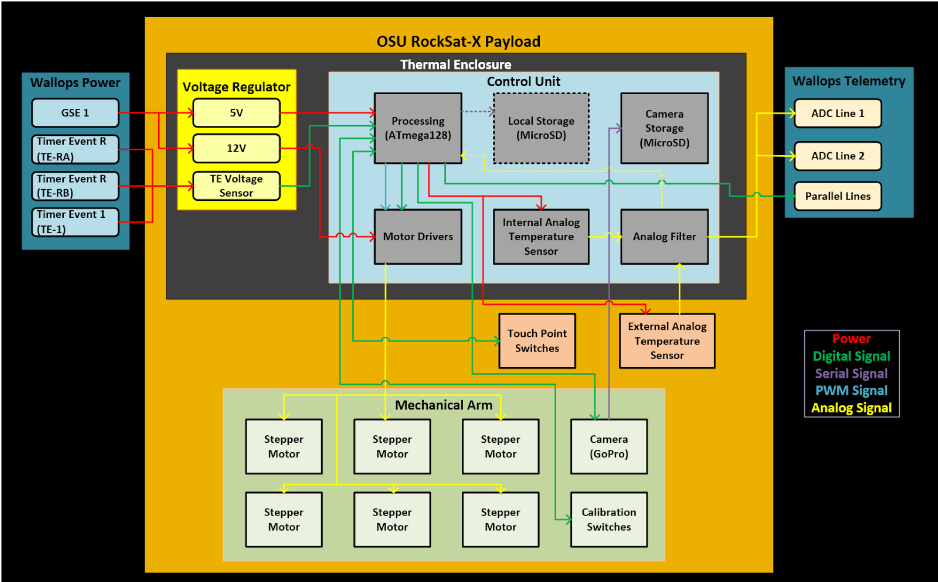
\includegraphics[width=\textwidth]{./images/ProjectDocs/functionalBlockDiagram}

\subsubsection{Flow Diagram}
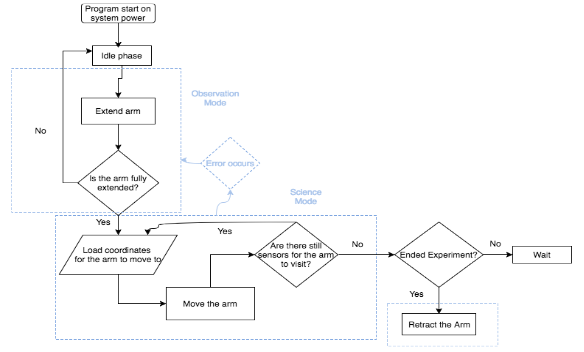
\includegraphics[width=\textwidth]{./images/ProjectDocs/flowDiagram}

\subsubsubsection{Pathing and Automation Subsystem Flow Diagram}
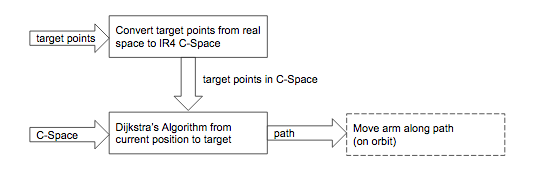
\includegraphics[width=\textwidth]{./images/ProjectDocs/pathingAndAutomationFlow}

\subsection{Hardware Requirements}
Minimum hardware requirements to run the software for the Hephaestus payload include:
\begin{itemize}
	\item{ATmega128 microcontroller}
	\item{USB ASP programmer}
\end{itemize}

\subsection{Installation Instructions}
To install the software on an ATmega128 chip, first ensure it is connected to
the computer with a USB ASP programmer. Then, from the 
\texttt{code/Hephaestus/Hephaestus} directory, run \texttt{make all}
followed by \texttt{make program}.

\subsection{Running Instructions}
The code will immediately begin running once the chip is powered on, and will
continue to run until power is lost.

\subsection{User Guides and Documentation}
TODO

